\documentclass[sigconf]{acmart}
% Cleaning 
\usepackage{pifont}
\usepackage{tabularx}
\pagestyle{fancy} % removes running headers
\settopmatter{printacmref=false} % Removes citation information below abstract
\renewcommand\footnotetextcopyrightpermission[1]{} % removes footnote with conference information in first column
\pagestyle{plain} % removes running headers
\fancyhead{}
\settopmatter{printacmref=false, printfolios=false}
% Copyright
\setcopyright{none}
% \setcopyright{acmcopyright}
% \setcopyright{acmlicensed}
% \setcopyright{rightsretained}
% \setcopyright{usgov}
% \setcopyright{usgovmixed}
% \setcopyright{cagov}
% \setcopyright{cagovmixed}
\settopmatter{printacmref=false} % Removes citation information below abstract
\acmDOI{}


\setlength{\parskip}{0pt}
\setlength{\parsep}{0pt}
\setlength{\headsep}{0pt}
\setlength{\topskip}{0pt}
\setlength{\topmargin}{0pt}
\setlength{\topsep}{0pt}
\setlength{\partopsep}{0pt}
%\linespread{0.95}
\usepackage{mdwlist}
\usepackage{amsmath}

\begin{document}
\title{SENG 474 Background and Related Work}
\author{Parris Mook-Sang-Forbes}
\affiliation{
  \institution{University of Victoria}
}
\email{parrisf@uvic.ca }
\author{Max Patchell}
\affiliation{
  \institution{University of Victoria}
}
\email{maxpatchell@uvic.ca}
\author{Varun Menon}
\affiliation{
  \institution{University of Victoria}
}
\email{varunmenon@uvic.ca}


\begin{abstract}
This paper follows the history of wildfire detection from horseback and aerial patrols, to today's automated, computerized detection methods. Current detection methods are split into two categories: sensor-based, and image-based (i.e., visual detection). Through process of elimination, we settle on deep convolutional neural networks (DCNNs) as a strong potential baseline on which to base our model, due to their flexibility and comparatively minimal tendency to falsely identify wildfires.
\end{abstract}
\keywords{Artifical Intelligence, Wildfires, Sensor Networks, Unmanned Aerial Vehicles, Neural Networks, Early Detection Systems}
\maketitle

%%----------Chapter 2------------------------------------------
\vspace{-1em}
\section{Introduction}
Despite breakthroughs in the field of early wildfire detection, there is more work to be done. Today's detection methods divide fire detection into a stark "fire" or "no fire" \cite{el-madafri}, without attempting to classify the fire's scale or severity. Additionally, these methods are prone to raising false positives, which could waste critical firefighting resources on a fire that doesn't exist. By comparing current detection methodologies, we hope to arrive on one that can serve as a viable baseline that can support our project throughout the term, while avoiding false positives.

\subsection{History}
Wildfire detection in North America used horseback patrols up until the First World War, aerial patrols being introduced after around 1920. Staffed lookout networks were expanded and became the dominant detection method by 1980.  By 2015, Alberta was the only remaining Canadian province that still relied on staffed lookout towers as part of its detection strategy \cite{fpi}. This transition reflected infrastructure maintenance costs, labour and safety standards, rather than being a shift based on detection performance alone: trained observers remained effective at identifying fires and estimating their characteristics. 

Human surveillance still faced limitations involving labour fatigue, reporting delays, visibility and limited coverage of remote forest areas. These constraints helped motivate the development of automated and remotely operated detection approaches. Modern approaches include satellite remote sensing, remotely piloted aircraft systems, and AI camera supported systems. These developments provided significant benefits for greater mobility and flexibility \cite{khan}. This evolution connects wildfire detection to computer science and machine learning through solving the problem of being able to accurately interpret observations and to identify evidence of fire \cite{fpi}.

\section{Prior Work}
We have broken down current wildfire detection methods into two main categories: sensor-based and camera/image-based (see: figure 1).

\begin{figure}[htp]
\caption{A taxonomy of current automated early wildfire detection systems}
\centering
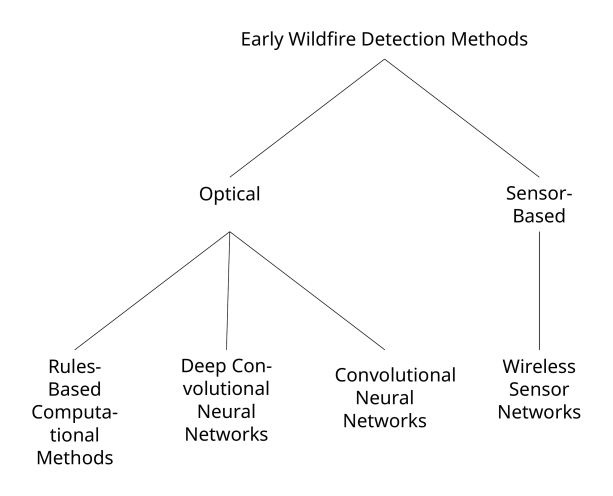
\includegraphics[width=0.5\textwidth]{heirarchy.png}
\end{figure}

\subsection{Sensor-Based and Multi-Modal Approaches}
Hardware-reliant data fusion systems heavily depend on distributed sensor and satellite networks. These setups require the deployment of wireless sensor networks (WSNs) to continuously record localized temperature, humidity, and smoke patterns, while also considering environmental variables alongside optical camera data \cite{bindal}. Similarly, satellite systems utilize thermal sensors to verify active hotspots \cite{bindal}. While these systems tend to be highly accurate in static environments, they are expensive to scale due to the cost of sensors and supporting devices. Furthermore, they are computationally heavy and struggle to adapt across diverse geographical regions \cite{bindal}.

\subsection{Camera and Image-Based Approaches}
\subsubsection{Rule-Based Methods}
Conversely, software-based systems utilize computer vision techniques, starting with rule-based computational models \cite{celik}. Early fire detection approaches utilized color spaces like RGB and YCbCr to separate luminance from chrominance, evaluating color moments to isolate flame pixels \cite{celik}. However, this method depends heavily on manual feature extraction and frequently triggers false alarms when encountering fire-like objects such as the sun, reddish foliage, or red flower clusters \cite{celik}. While color-based models are generally inexpensive, they rely on ideal environmental lighting and struggle to adapt to dynamic outdoor conditions \cite{celik}.

\subsubsection{Single-Task Deep Learning}
To overcome these visual limitations, modern systems employ deep convolutional neural networks (DCNNs) using unmanned aerial vehicle (UAV) imagery \cite{zhao}. Directly resizing high-resolution, wide-angled aerial images into fixed deep learning inputs causes geometric distortion and detail loss, often submerging critical fire features into background clutter \cite{zhao}. By applying saliency detection algorithms, systems can rapidly localize and segment the core fire area before resizing, preserving the structural integrity of flame and smoke features for training the neural network \cite{zhao}. DCNNs, such as the 15-layer fire-net architecture, automatically learn high-level sparse features to distinguish irregular fire boundaries from cluttered backgrounds without relying on manual feature descriptors \cite{zhao}. Ultimately, UAVs equipped with visible spectrum cameras offer a highly adaptable, low-cost surveillance alternative to expensive and geographically limited thermal imaging systems \cite{zhao}.

\subsection{Multi-Task Deep Learning}
Despite these advancements, aerial visual detection faces complex environmental challenges that require a multi-tasking approach \cite{el-madafri}. Atmospheric phenomena like fog, mist, and low-altitude clouds frequently produce illusions of smoke due to their translucent and diffused appearance \cite{el-madafri}. Lighting variations from the sun's angle or reflections off water and wet trees produce bright spots that mimic active fires, while seasonal changes like red and orange foliage can be easily mistaken for flames or embers \cite{el-madafri}. Additionally, camera motion blur and platform vibrations from the UAVs introduce artifacts that resemble smoke or fire, further complicating automated detection \cite{el-madafri}. Hence, standard binary classification convolutional neural networks (CNNs) are forced to output a simple "fire" or "no fire" prediction, which leads to higher false-positive rates when the network encounters complex visual confounding variables \cite{el-madafri}.

\subsection{Comparative Analysis}
Although today's wildfire detection methods utilize sophisticated censors and neural networks, some are still susceptible to some of the same limitations as their horseback ancestors: optical detection methods run the risk of misinterpreting visual information. Detection methods utilizing Rule-based computational models and CNNs are especially prone to conflating actual wildfires with superficially similar visual information (e.g., red-coloured image areas) \cite{celik}\cite{el-madafri}. We seek to avoid these kinds of false positives, so we can discount these detection methods as potential baselines to iterate upon.

We must also acknowledge that certain detection methods fall outside the scope of our project limitations. CNNs are conceptually incompatible with our goals; they can only make a binary, "fire" or "no fire" judgment call \cite{el-madafri}, which is incompatible with our project goals (see: section 2.5). Because we only have a limited time-frame to explore solutions, we must eliminate a sensor-based approach, as it would require us to construct a simulated model of a WSN. 

After eliminating all other options (see: table 1), our only viable option left is single-task deep learning. DCNNs are a flexible solution that have a lower baseline for false positive detections. 

\begin{table}[]
\centering
\begin{tabularx}{\columnwidth}{X|X|X|X}
\hline
 & Compatible w/ Goals & Logistically Feasible & Doesn't Raise False Positives \\ \hline
WSN & Y & N & Y \\
Rule-Based & Y & N & N \\
DCNN & Y & Y & Y \\
CNN & N & Y & N \\ \hline
\end{tabularx}
\caption{Using process of elimination on our selected methods.}
\end{table}

\subsection{Contextualizing our Project}
Our project investigates machine-learning-based classification of aerial wildfire images. Given a single image, our proposed model assigns one of three apparent risk levels: low, medium or high. Within the categories reviewed, it falls under software-based computer vision, with convolutional neural networks for aerial imagery and multi-task fire and smoke analysis being the most closely related approaches. These methods inform our investigation of how visual features can distinguish wildfire evidence from ambiguous environmental features such as fog, clouds, sunlight reflections, and foliage.

Our intended contribution is to investigate whether a three-class model can distinguish apparent risk levels while limiting misclassifications caused by misleading environmental features. Reducing these misclassifications could help prevent unnecessary allocation of vital firefighting resources. The project's effectiveness will therefore depend on both its classification performance and its ability to avoid assigning elevated risk to images containing such features. 


\bibliographystyle{ACM-Reference-Format}
\begin{thebibliography}{9}
\bibitem{fpi}
FPInnovations. 2022. The faster (the response) the better: The evolution of wildfire detection solutions. Retrieved from https://web.fpinnovations.ca/the-faster-the-response-the-better-the-evolution-of-wildfire-detection-solutions/.
\bibitem{khan}
Alimul Haque Khan, Ali Newaz Bahar, and Khan Wahid. 2025. A Review on Forest Fire Detection Techniques: Past, Present, and Sustainable Future \emph{Sensors} 14, 2 (March 2026) https://doi.org/10.3390/s26051609.
\bibitem{bindal}
Rohi Bindal, Shubhangi Deokar, Trilochan Singh Rathore, Aditi Sharma, Rupali Gangarde, and Ashwini Jatti. 2024. AI-ML Innovations in Forest Fire Detection: Protecting Ecosystems and Communities. In \emph{2024 International Conference on Computing, Sciences and Communications (ICCSC)} October 24 - 25, 2024, Ghaziabad, India. 10.1109/ICCSC62048.2024.10830309
\bibitem{celik}
Çelik Turgay, Demirel Hasan. 2009. Fire detection in video sequences using a generic color model. \emph{Fire Safety Journal} 44, 2 (February 2009), 147-1589. https://doi.org/10.1016/j.firesaf.2008.05.005.
\bibitem{zhao}
Yi Zhao, Jiale Ma, Xiaohui Li, Jie Zhang. 2018. Saliency Detection and Deep Learning-Based Wildfire Identification in UAV Imagery. \emph{Sensors} 18, 3 (February 2018) https://doi.org/10.3390/s18030712.
\bibitem{el-madafri}
Ismail El-Madafri, Marta Peña, and Noelia Olmedo-Torre. 2023. The Wildfire Dataset: Enhancing Deep Learning-Based Forest Fire Detection with a Diverse Evolving Open-Source Dataset Focused on Data Representativeness and a Novel Multi-Task Learning Approach. \emph{Forests} 14, 9 (August 2023) https://doi.org/10.3390/f14091697.
\end{thebibliography}

\end{document}

